\documentclass[a4paper,10pt]{article} 
\usepackage[utf8]{inputenc}
\usepackage[a4paper]{geometry}
\usepackage[magyar]{babel}
\usepackage{t1enc}
\usepackage{amsmath}
\usepackage{amssymb}
\usepackage{pgf,tikz,longtable}
\usetikzlibrary{arrows}
\frenchspacing 
\pagestyle{empty}
\newcommand{\ki}[2]{\hfill {\it #1 (#2)}\medskip}
\newcommand{\vonal}{\hbox to \hsize{\hskip2truecm\hrulefill\hskip2truecm}}
\newcommand{\degre}{\ensuremath{^\circ}}
\newcommand{\tg}{\mathop{\mathrm{tg}}\nolimits}
\newcommand{\ctg}{\mathop{\mathrm{ctg}}\nolimits}
\newcommand{\arc}{\mathop{\mathrm{arc}}\nolimits}
\begin{document}
\begin{center} \Large {\em 23. Nemzetközi Magyar Matematika Verseny} \end{center}
\begin{center} \large{\em Csíkszereda, 2014. március 12-16.} \end{center}
\smallskip
\begin{center} \large{\bf 9. osztály} \end{center}
\bigskip 

{\bf 1. feladat: } Egy könyvtárban megszámozták az összes könyvet. A
számozáshoz $1$-től kez\-dő\-dő\-en egymást követő
természetes szá\-mo\-kat használtak, és ugyanazt a számot
nem írták rá két könyvre. A megszámozás során a
könyvekre háromszor annyi számjegyet kellett
ráírni, mint ahány könyv volt a könyvtárban.
Hány könyv volt a könyvtárban?

\ki{\fbox{Oláh György}}{Révkomárom}\medskip

{\bf 1. megoldás: } Legyen a keresett kötetek száma $x$. Ez a
szám nem lehet egyjegyű, mert $x>0$ esetén $x\neq3x$. Ha
$x$ kétjegyű, akkor $9+2(x-9)=3x,$ mert az egyjegyű
számjegyek száma $9$, a kétjegyű számok
számjegyeinek száma pedig $2(x-9)$. Ennek az egyenletnek
nincs megoldása a természetes számok halmazán.

Ha $x$ háromjegyű, akkor $9+2\cdot90+3(x-99)=3x,$ és
ennek az egyenletnek sincs megoldása.

Ha $x$ négyjegyű, akkor az egyenlet:
\[
9+2\cdot90+3\cdot900+4(x-999)=3x,%
\]
és ennek az egyetlen megoldása $x=1107$.

 Ha a kötetek
száma $1107+y$ is lehetne, ahol $y$ pozitív egész,
akkor a könyvek megjelölésére legalább
$3\cdot1107+4y$ számjegyet kellene felhasználni. (Az első
1107 kötethez $3\cdot 1107$ számjegyet és minden további
kötethez legalább $4$ számjegyet.) Másrészt $y>0$ esetén
$3\cdot1107+4y>3(1107+y),$ tehát $1107$ az egyedüli
megoldása a feladatnak.

\medskip

{\bf 2. megoldás: } Legyen a keresett kötetek száma $x$. Jelöljük az $x$
szám számjegyeinek számát $(k+1)$-gyel. Ekkor az
előbbiekben is felírtuk, hogy $k\geq1$ (azaz a szám
legalább kétjegyű kell legyen) és a számozás
során felhasznált számjegyek száma:
$$9+2\cdot90+3\cdot900+\ldots+k\cdot9\cdot10^{k-1}+(k+1)(x-10^{k}+1).
$$
Az első összeget a következőképpen alakíthatjuk:
$$9\left(  1+2\cdot10+3\cdot10^{2}+\ldots+k\cdot10^{k-1}\right)=$$
$$9\left[  \left(  1+\ldots+10^{k-1}\right)  +10\left(  1+
\ldots+10^{k-2}\right)  +\ldots+10^{k-1}\right]=$$ $$9\left[
\frac{10^{k}-1}{9}+10\cdot\frac{10^{k-1}-1}{9}+\ldots+10^{k-1}\cdot\frac{10-1}{9}\right]=$$
$$\left[  \left(  10^{k}-1\right)  +\left( 10^{k}-10\right) +\ldots+\left( 10^{k}-10^{k-1}\right) \right]
=$$ $$ k\cdot10^{k}-\frac{10^{k}-1}{9},$$ tehát a számjegyek
száma
$$ k+(k+1)x-\frac{10^{k+1}-10}{9}.%
$$
Így
\[
3x=k+(k+1)x-\frac{10^{k+1}-10}{9},%
\]
azaz
\[
(k-2)x=\frac{10(10^{k}-1)}{9}-k,%
\]
vagy
\[
(k-2)x={\underbrace{111\ldots1}_{k \mbox{ darab}}0}-k.%
\]
A fenti összefüggés jobb oldala egy $1$-gyel
kezdődő $(k+1)$-jegyű szám. A bal oldalon ott van a
$(k+1)$-jegyű $x$ és így $k>3$ esetén a baloldal
nem lehet $1$-gyel kezdődő $(k+1)$-jegyű szám. A
$k=3$ esetben pedig $x=1107$.

\medskip


\vonal


{\bf 2. feladat: } Határozd meg az $(a+b)(b+c)(c+a)=1144$ egyenlet összes
nullától különböző természetes megoldását!

\ki{dr.~Hraskó András}{Budapest}\medskip

{\bf Megoldás: }  $1144=8\cdot 11\cdot 13.$ Mivel az $(a+b)$, $(b+c)$, $(c+a)$ tényezők
összege páros, ha közülük kettő páros, akkor a
harmadik is az. Így vagy csak egyikük páros, vagy mind
párosak.

Ha mind párosak, akkor legalább az egyik közülük $2,$
mert a prímtényezős felbontásban nincs három páratlan
prím. Mivel $2$ egyetlen felbontása pozit\'{i}v egészek
összegére az $1+1$, a szorzat további két tényezője
egymással egyenlő lenne. Ez nem lehetséges, tehát ebben az
esetben nincs megoldás.

Ha csak egyikük páros, akkor szükségképpen $8$,
$11$ és $13$ a három kéttagú összeg, tehát a
számok valamilyen sorrendben $3$, $5$ és $8$.

\medskip

\vonal


{\bf 3. feladat: } Az $ABCD$ konvex négyszögben $AB=1,$ $BC=2,$ $AD = \sqrt{2}$,
$A\sphericalangle = 105^{\circ}$ és $B\sphericalangle  = 60^\circ$.
Számítsd ki a $CD$ oldal hosszát!


\ki{Kovács Lajos}{Székelyudvarhely}

\ki{dr.~András Szilárd}{Kolozsvár}\medskip

{\bf 1. megoldás: } Jelöljük a $DC$ oldal hosszát $x$-szel és a $BC$ oldal felező\-pont\-ját $M$-mel.
    \begin{center}
        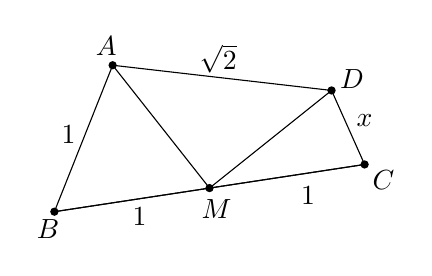
\begin{tikzpicture}[line cap=round,line join=round,>=triangle 45,x=1.0cm,y=1.0cm]
%\clip(-8.64,-2) rectangle (18.68,1);
\draw (-1.54,0.64)-- (-2.28,-1.22); \draw (-2.28,-1.22)--
(1.66,-0.62); \draw (1.66,-0.62)-- (1.24,0.32); \draw (1.24,0.32)--
(-1.54,0.64); \draw (-1.54,0.64)-- (-0.31,-0.92); \draw
(-0.31,-0.92)-- (1.24,0.32); \draw (-2.28,-1.22)-- (-0.31,-0.92);
\draw (-0.31,-0.92)-- (1.66,-0.62);
%\begin{scriptsize}
\fill [color=black] (-1.54,0.64) circle (1.5pt); \draw[color=black]
(-1.62,0.88) node {$A$}; \fill [color=black] (-2.28,-1.22) circle
(1.5pt); \draw[color=black] (-2.36,-1.44) node {$B$}; \fill
[color=black] (1.66,-0.62) circle (1.5pt); \draw[color=black]
(1.9,-0.82) node {$C$}; \fill [color=black] (1.24,0.32) circle
(1.5pt); \draw[color=black] (1.5,0.46) node {$D$};
\draw[color=black] (-2.1,-0.24) node {$1$}; \draw[color=black]
(1.66,-0.06) node {$x$}; \draw[color=black] (-0.2,0.72) node {$\sqrt
2$}; \fill [color=black] (-0.31,-0.92) circle (1.5pt);
\draw[color=black] (-0.22,-1.18) node {$M$}; \draw[color=black]
(-1.2,-1.28) node {$1$}; \draw[color=black] (0.94,-1.02) node {$1$};
\end{tikzpicture}
    \end{center}
    A feltételek alapján $BM= MC = 1$, tehát az $ABM$ háromszög egyenlő oldalú,
    és ezért $MAD\sphericalangle = 45^\circ.$ Az $MAD$ háromszögben viszont
    $AD = \sqrt{2}$ és $AM=1$ is teljesül, így az $MAD$ háromszög $M$-ben derékszögű
     és egyenlő szárú, tehát $MD=1.$ Következik, hogy $DMC\sphericalangle = 180^\circ - 60^\circ-90^\circ = 30^\circ$.
      Tehát a $DMC$ háromszög egyenlő szárú, $DM = MC = 1$ és
      az
      $M$ csúcsnál levő szög $30^{\circ}$-os. Ha ebben a háromszögben
      felvesszük az $M$ csúcsból kiinduló magasságot (ami egyben szögfelező és oldalfelező is), akkor következik, hogy
    \[
        x = 2\sin15^\circ = 2\sqrt{\frac{1-\cos30^\circ}{2} } = \sqrt2\cdot \sqrt{1- \frac{\sqrt3}{2}} = \sqrt{2-\sqrt{3}}.
    \]

\medskip

{\bf 2. megoldás: } Jelöljük a $DC$ oldal hosszát $x$-szel, a $BC$ oldal felezőpontját $M$-mel,
     és az $AD$ és $BC$ egyenesek metszéspontját $N$-nel.
    \begin{center}
    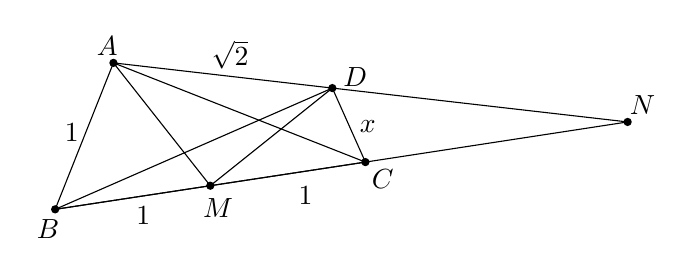
\begin{tikzpicture}[line cap=round,line join=round,>=triangle 45,x=1.0cm,y=1.0cm]
%\clip(-3.8, -0.5) rectangle (17.45,2.36);
\draw (0.96,2.04)-- (0.22,0.18); \draw (0.96,2.04)-- (4.16,0.78);
\draw (0.22,0.18)-- (4.16,0.78); \draw (0.22,0.18)-- (3.74,1.72);
\draw (4.16,0.78)-- (3.74,1.72); \draw (3.74,1.72)-- (0.96,2.04);
\draw (0.96,2.04)-- (2.19,0.48); \draw (2.19,0.48)-- (3.74,1.72);
\draw (0.22,0.18)-- (2.19,0.48); \draw (2.19,0.48)-- (4.16,0.78);
\draw (3.74,1.72)-- (7.49,1.29); \draw (7.49,1.29)-- (4.16,0.78);
\fill [color=black] (0.96,2.04) circle (1.5pt); \draw[color=black]
(0.88,2.25) node {$A$}; \fill [color=black] (0.22,0.18) circle
(1.5pt); \draw[color=black] (0.13,-0.07) node {$B$}; \fill
[color=black] (4.16,0.78) circle (1.5pt); \draw[color=black]
(4.38,0.57) node {$C$}; \fill [color=black] (3.74,1.72) circle
(1.5pt); \draw[color=black] (4.03,1.86) node {$D$};
\draw[color=black] (0.43,1.16) node {$1$}; \draw[color=black]
(4.19,1.23) node {$x$}; \draw[color=black] (2.44,2.14) node {$\sqrt
2$}; \fill [color=black] (2.19,0.48) circle (1.5pt);
\draw[color=black] (2.29,0.2) node {$M$}; \draw[color=black]
(1.34,0.1) node {$1$}; \draw[color=black] (3.4,0.36) node {$1$};
\fill [color=black] (7.49,1.29) circle (1.5pt); \draw[color=black]
(7.68,1.5) node {$N$};
\end{tikzpicture}
    \end{center}
      Az előző megoldáshoz hasonlóan megkapjuk, hogy  
      $BCD\sphericalangle = 75^\circ$
    és $CDA\sphericalangle = 75^\circ + 45^\circ = 120^\circ$. Tehát az $ABCD$ négyszög
    szemközti szögeinek az összege $180^\circ$ és így a négyszög körbeírható.
    A négy\-szög köré írt kör középpontja az $M$ pont (és a kör sugara $1$),
     ezért a $BAC\sphericalangle$ és $BDC\sphericalangle$ szögek $90^{\circ}$-osak. Pitagorasz tétele
     alapján az
    \begin{equation}\label{eq:2}
        AC = \sqrt 3 \quad \mbox{és} \quad   x^2 = 4-BD^2
    \end{equation}
    összefüggéseket kapjuk.

    Másrészt, $AMD\sphericalangle = 90^\circ$, $BMA\sphericalangle = 60^\circ$ és a
    $BMD$ háromszög egyenlő szárú, tehát   $MBD\sphericalangle = 15^\circ.$
     Viszont az $ABCD$ négyszög körbeírható, ezért a $CAD\sphericalangle$ is $15^{\circ}.$ De az $ANB$ háromszögben az $ANB\sphericalangle$ is $15^{\circ}$-os
     így az $ACN$ háromszög egyenlő szárú és
    \begin{equation}\label{eq:3}
    CN = AC = \sqrt{3}
    \end{equation}
     az (\ref{eq:2}) összefüggés alapján.

    Mivel a $BDN$ háromszög is egyenlő szárú (a $BN$ oldalon fekvő szögek $15^{\circ}$-osak), ezért
    \begin{equation}\label{eq:4}
        BD = DN = y.
    \end{equation}
    Ha felírjuk az $N$ pontnak az $ABCD$ négyszög köré írt körre vonatkozó
     hatványát (vagy direkt hasonlóságból), a (\ref{eq:3}) és (\ref{eq:4}) összefüggések
     alapján az
    \[
    ND\cdot NA = NC\cdot NB \quad \Longleftrightarrow \quad y(y+\sqrt2) = \sqrt3(\sqrt3 + 2)
    \]
    összefüggéshez jutunk. Az $y$-ban másodfokú egyenletnek csak az egyik megoldása
    lesz pozitív (csak ez lehet egyenlő egy szakasz hosszával), és mivel $BD = y$, az (\ref{eq:2}) egyenletből megkapjuk az $x$ értékét.

\medskip

{\bf 3. megoldás: }   Legyen a $DC$ szakasz hossza $x$, a $BC$ oldal felezőpontja $M$, a $DCM$ háromszög $D$-ből húzott magasságának a hossza $h$ és ez a magasság a $CM$ szakaszt ossza $y$ és $1-y$ részekre (lásd az ábrát).
    \begin{center}
    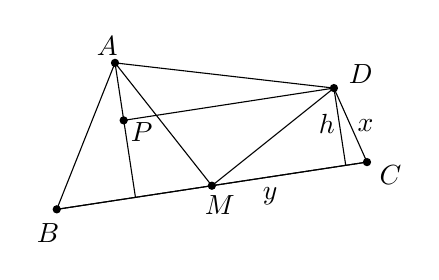
\begin{tikzpicture}[line cap=round,line join=round,>=triangle 45,x=1.0cm,y=1.0cm]
%\clip(-5.65,-0.6) rectangle (20.34,2.45);
\draw (0.96,2.04)-- (0.22,0.18); \draw (0.22,0.18)-- (4.16,0.78);
\draw (4.16,0.78)-- (3.74,1.72); \draw (3.74,1.72)-- (0.96,2.04);
\draw (0.96,2.04)-- (2.19,0.48); \draw (2.19,0.48)-- (3.74,1.72);
\draw (0.22,0.18)-- (2.19,0.48); \draw (2.19,0.48)-- (4.16,0.78);
\draw (0.96,2.04)-- (1.22,0.33); \draw (1.07,1.31)-- (3.74,1.72);
\draw (3.74,1.72)-- (3.89,0.74); \fill [color=black] (0.96,2.04)
circle (1.5pt); \draw[color=black] (0.86,2.25) node {$A$}; \fill
[color=black] (0.22,0.18) circle (1.5pt); \draw[color=black]
(0.11,-0.12) node {$B$}; \fill [color=black] (4.16,0.78) circle
(1.5pt); \draw[color=black] (4.46,0.62) node {$C$}; \fill
[color=black] (3.74,1.72) circle (1.5pt); \draw[color=black]
(4.08,1.9) node {$D$}; \draw[color=black] (2.93,0.35) node {$y$};
\draw[color=black] (4.14,1.25) node {$x$};
%\draw[color=black] (2.93,2.09) node {$\sqrt 2$};
\fill [color=black] (2.19,0.48) circle (1.5pt); \draw[color=black]
(2.29,0.24) node {$M$}; \fill [color=black] (1.07,1.31) circle
(1.5pt); \draw[color=black] (1.3,1.16) node {$P$};
\draw[color=black] (3.65,1.27) node {$h$};
\end{tikzpicture}
    \end{center}
    Az első megoldáshoz hasonlóan $DM = 1$ és ezért Pitagorasz tétele alapján a
    \begin{equation} \label{eq:5}
        h^2 + y^2 = 1 \quad \mbox{és} \quad h^2 + (1-y)^2 = x^2
    \end{equation}
    egyenletekhez jutunk.

    Szükségünk van még egy egyenletre, ezért rajzoljuk be az $ABM$ egyenlő oldalú
    háromszögben az $A$ csúcsból húzott magasságot (aminek a hossza $\frac{\sqrt{3}}{2}$),
     majd állítsunk a $D$ pontból egy merőlegest erre a magasságra (és jelöljük
     ennek talppontját $P$-vel, lásd az ábrát). A harmadik egyenletünket az $APD$
     derékszögű háromszögben felírt Pitagorasz tételből kapjuk:
    \begin{equation}\label{eq:6}
        \left( \frac{\sqrt{3}}{2} -h \right)^2 + \left( \frac{1}{2} + y \right)^2 = (\sqrt{2})^2.
    \end{equation}
    A fenti három egyenletből átalakításokkal a
    \begin{eqnarray*}
        2 - 2y &=&x^2,\\
        h^2 + y^2 &=&1,\\
        \sqrt3 h &=& y
    \end{eqnarray*}
    egyenleteket kapjuk (a $h^2+y^2=1$ összefüggést használtuk a másik két egyenlet egy\-sze\-rű\-sí\-té\-sé\-re, az utolsó egyenlet
    felírható a $30^{\circ}$-os szög tangenséből is).
    Az utolsó két egyenletből következik, hogy
    $h=\frac 12$ és így $y=\frac{\sqrt{3}}{2},$ tehát az első egyenletből következik, hogy
    $x=\sqrt{2-\sqrt{3}}.$

\medskip

\textit{Megjegyzés}: A mellékelt ábra alapján látható, hogy
lépésről-lépésre csak a Pitagorasz tétel
alkalmazásával is kiszámolható a kért szakasz hossza.

\begin{center}
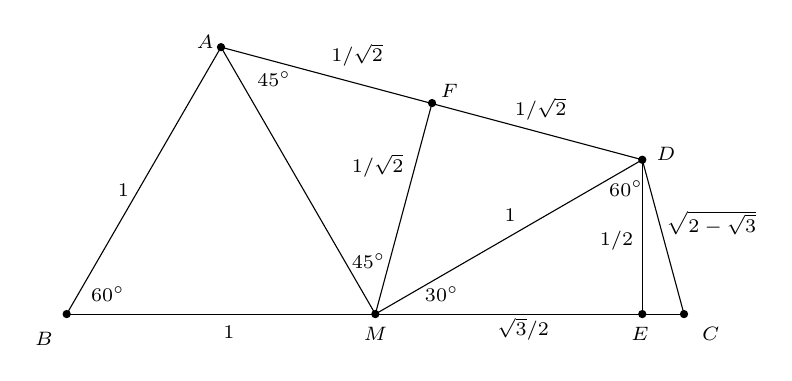
\begin{tikzpicture}[line cap=round,line join=round,>=triangle 45,x=1.0cm,y=1.0cm]
\draw (-4.92,4)-- (2.92,4); \draw (-4.92,4)-- (-2.96,7.39); \draw
(-2.96,7.39)-- (2.39,5.96); \draw (2.39,5.96)-- (2.92,4); \draw
(-1,4)-- (2.39,5.96); \draw (-1,4)-- (-2.96,7.39); \draw
(-0.28,6.68)-- (-1,4); \draw (2.39,4)-- (2.39,5.96); \draw
(2.92,4)-- (-4.92,4);
\begin{scriptsize}
\fill [color=black] (-4.92,4) circle (1.5pt); \draw (-4.71,4.45)
node[anchor=north west] {$60^\circ$}; \draw (-4.37,5.75)
node[anchor=north west] {$1$}; \draw (-0.47,4.45) node[anchor=north
west] {$30^\circ$}; \draw (-2.6,7.18) node[anchor=north west]
{$45^\circ$}; \draw (-1.40,4.87) node[anchor=north west]
{$45^\circ$}; \draw (-3.03,3.95) node[anchor=north west] {$1$};
\draw (1.87,5.79) node[anchor=north west] {$60^\circ$}; \draw
(-1.66,7.53) node[anchor=north west] {$1/\sqrt{2}$}; \draw
(-1.4,6.13) node[anchor=north west] {$1/\sqrt{2}$}; \draw
(0.67,6.85) node[anchor=north west] {$1/\sqrt{2}$}; \draw
(0.45,4.05) node[anchor=north west] {$\sqrt{3}/2$}; \draw
(0.54,5.44) node[anchor=north west] {$1$}; \draw (1.75,5.15)
node[anchor=north west] {$1/2$}; \draw (2.6,5.41) node[anchor=north
west] {$\sqrt{2-\sqrt{3}}$}; \draw[color=black] (-5.21,3.69) node
{$B$}; \fill [color=black] (-1,4) circle (1.5pt); \draw[color=black]
(-1,3.75) node {$M$}; \fill [color=black] (-2.96,7.39) circle
(1.5pt); \draw[color=black] (-3.16,7.46) node {$A$}; \fill
[color=black] (2.92,4) circle (1.5pt); \draw[color=black]
(3.26,3.75) node {$C$}; \fill [color=black] (2.39,5.96) circle
(1.5pt); \draw[color=black] (2.69,6.03) node {$D$}; \fill
[color=black] (-0.28,6.68) circle (1.5pt); \draw[color=black]
(-0.06,6.84) node {$F$}; \fill [color=black] (2.39,4) circle
(1.5pt); \draw[color=black] (2.36,3.75) node {$E$};
\end{scriptsize}
\end{tikzpicture}
\end{center}

\medskip

\vonal


{\bf 4. feladat: } Hány valós megoldása van a $3\left[  x\right]
=2x^{2}+x-4$ egyenletnek? ($\left[  x\right]  $ az $x$ valós
szám egész részét jelenti.)

\ki{Szabó Magda}{Szabadka}

\ki{Longáver Lajos}{Nagybánya}\medskip

{\bf 1. megoldás: }  Mivel $x-1<\left[  x\right]  \leq x$, a következő
egyenlőtlenségekhez jutunk:
\[
3\left(  x-1\right)  <2x^{2}+x-4\leq3x.
\]


Az így kapott egyenlőtlenségeket megoldjuk:
\[
\left\{
\begin{array}
[c]{c}%
2x^{2}-2x-1>0\\
2x^{2}-2x-4\leq0
\end{array}
\right.  \Leftrightarrow\left\{
\begin{array}
[c]{c}%
x\in\left(  -\infty,\frac{1-\sqrt{3}}{2}\right)  \cup\left(  \frac{1+\sqrt{3}%
}{2},+\infty\right) \\
x\in\left[  -1,2\right]
\end{array}
\right.  \]

Tehát $x\in\left[ -1,\frac{1-\sqrt{3}}{2}\right) \cup\left(
\frac{1+\sqrt{3}}{2},2\right]$ és így $\left[  x\right]
\in\left\{  -1,1,2\right\}  $.

Ha $\left[  x\right]  =-1$, akkor a feladatbeli egyenlet
$2x^{2}+x-1=0$, és ennek az egyetlen olyan megoldása,
amelynek az egészrésze $-1$, az $x=-1$. (A másik
megoldás $\frac{1}{2}$, ennek viszont az egészrésze
$0$.)

Ha $\left[  x\right]  =1$, akkor a feladatbeli egyenlet
$2x^{2}+x-7=0$, és ennek az egyetlen olyan megoldása,
amelynek az egészrésze $1$, az a $x=\frac{-1+\sqrt{57}}{4}$.
(A másik megoldás $\frac {-1-\sqrt{57}}{4}$.)

Ha $\left[  x\right]  =2$, akkor a feladatbeli egyenlet
$2x^{2}+x-10=0$, és ennek az egyetlen olyan megoldása,
amelynek az egészrésze $2$, az $x=2$. (A másik
megoldás $-\frac{5}{2}$.)

A fentieket összefoglalva, az egyenletnek összesen $3$
megoldása van, ezek pedig a $-1,\frac{-1+\sqrt{57}}{4}$ és a
$2$.

\medskip

{\bf 2. megoldás: } 
Ábrázoljuk az $y=\frac{2}{3}x^{2}+\frac{1}{3}x-\frac{4}{3}$
egyenletű parabolát, majd az $y=\left[  x\right]  $
függvény grafikus képét.

\begin{center}
\begin{tikzpicture}[line cap=round,line join=round,>=triangle 45,x=1.0cm,y=1.0cm]
\draw[->,color=black] (-4,0) -- (4,0); \foreach \x in
{-4,-3,-2,-1,1,2,3} \draw[shift={(\x,0)},color=black] (0pt,2pt) --
(0pt,-2pt) node[below] {\footnotesize $\x$}; \draw[->,color=black]
(0,-1.5) -- (0,3.5); \foreach \y in {-1,1,2,3}
\draw[shift={(0,\y)},color=black] (2pt,0pt) -- (-2pt,0pt) node[left]
{\footnotesize $\y$}; \draw[color=black] (0pt,-10pt) node[right]
{\footnotesize $0$}; \clip(-4,-1.5) rectangle (4,3.5);
\draw[smooth,samples=100,domain=-4.0:4.0]
plot(\x,{2/3*(\x)^2+1/3*(\x)-4/3}); \draw [line width=1.2pt] (0,0)--
(1,0); \draw [line width=1.2pt] (1,1)-- (2,1); \draw [line
width=1.2pt] (2,2)-- (3,2); \draw [line width=1.2pt] (3,3)-- (4,3);
\draw [line width=1.2pt] (-1,-1)-- (0,-1);
\begin{scriptsize}
\fill [color=black] (2,2) circle (1.5pt); \fill [color=black]
(-1,-1) circle (1.5pt); \fill [color=black] (1.64,1) circle (1.5pt);
\end{scriptsize}
\end{tikzpicture}
   \end{center}
Az ábra alapján látható, hogy a megoldások $-1,2$ és egy
$(1,2)$ intervallumbeli szám. Mivel a feladat nem kéri
konkrétan a megoldásokat, csak a megoldások
számát, ezért ez elégséges is. Hasonló, de talán
jobban látható gondolatmenethez jutunk, ha az egészrész
függvény helyett a törtrész függvény grafikus képét
ábrázoljuk. Ehhez átalakítjuk az egyenletet: \[3\left[
x\right]  =2x^{2}+x-4\Leftrightarrow3\left(  x-\left\{ x\right\}
\right)  =2x^{2}+x-4,\] tehát a
$\displaystyle \left\{  x\right\}  =-\frac{2}{3}%
x^{2}+\frac{2}{3}x+\frac{4}{3} $ egyenlethez jutunk.
Ha ábrázoljuk az $y=-\frac{2}{3}x^{2}+\frac{2}{3}x+\frac{4}%
{3}$ egyenletű parabolát, majd az $y=\left\{  x\right\}  $
függvényt. \'{I}gy sokkal jobban látszik a három
megoldás.

\begin{center}
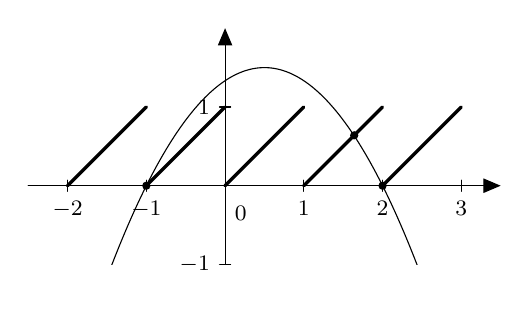
\begin{tikzpicture}[line cap=round,line join=round,>=triangle 45,x=1.0cm,y=1.0cm]
\draw[->,color=black] (-2.5,0) -- (3.5,0); \foreach \x in
{-2,-1,1,2,3} \draw[shift={(\x,0)},color=black] (0pt,2pt) --
(0pt,-2pt) node[below] {\footnotesize $\x$}; \draw[->,color=black]
(0,-1) -- (0,2); \foreach \y in {-1,1}
\draw[shift={(0,\y)},color=black] (2pt,0pt) -- (-2pt,0pt) node[left]
{\footnotesize $\y$}; \draw[color=black] (0pt,-10pt) node[right]
{\footnotesize $0$}; \clip(-2.5,-1) rectangle (3.5,2);
\draw[smooth,samples=100,domain=-2.5:3.5]
plot(\x,{(-2)/3*(\x)^2+2/3*(\x)+4/3}); \draw [line width=1.2pt]
(0,0)-- (1,1); \draw [line width=1.2pt] (1,0)-- (2,1); \draw [line
width=1.2pt] (2,0)-- (3,1); \draw [line width=1.2pt] (-1,0)-- (0,1);
\draw [line width=1.2pt] (-2,0)-- (-1,1);
\begin{scriptsize}
\fill [color=black] (2,0) circle (1.5pt); \fill [color=black] (-1,0)
circle (1.5pt); \fill [color=black] (1.64,0.64) circle (1.5pt);
\end{scriptsize}
\end{tikzpicture}
\end{center}
\vspace*{-1cm}

\medskip

{\bf 3. megoldás:} Tekintsük az  $f\left(  x\right)  =2x^{2}+x-\left(  4+3k\right)
$ függ\-vényt, ahol $k=\left[  x\right]  .$

Ha $x\leq-2$, akkor $f\left(  x\right)  =x(x+2)-(4+3k)>0$.

Az $f$ függvény minden $x\in\left(  0,-\frac{1}{4}\right)  $
esetén szigorúan csökkenő, ha pedig $x\in\left(  -\frac{1}%
{4},+\infty\right)  $, akkor szigorúan növekvő.

Ha $x\in\left(  -\frac{1}{4},+\infty\right)  $, akkor - mivel
szigorúan növekvő - $f$-nek minden $\left[  k,k+1\right)
$ intervallumban legfennebb egy gyöke van. Ez a gyök
pontosan akkor létezik, ha $f\left(  k\right)  \leq0$ és
$f\left(  k+1-\epsilon\right)  >0$, ha $\epsilon$ elég kicsi. Ha
$\epsilon\rightarrow0$, akkor $$f\left( k+1-\epsilon\right)
\rightarrow2\left(  k+1\right)  ^{2}+\left(  k+1\right)
-(4+3k)=2k^{2}+2k-1$$ és ez nullánál szigorúan
nagyobb kellene legyen.

Az $f\left(  k\right)
\leq0\Leftrightarrow2k^{2}-2k-4\leq0\Leftrightarrow k\in\left\{
-1,0,1,2\right\}  $. \newline A $2k^{2}+2k-1>0$
egyenlőtlenség viszont csak $k=1$ és $k=2$ esetén
teljesül.

Ha $x\in\left(  -2,-\frac{1}{4}\right)  $, akkor $k\in\left\{
-2,-1\right\} $ és $f$ szigorúan csökkenő. A $k=-2$
és $k=-1$ értékeket egyszerű
visszahelyettesítéssel ellenőrizhetjük. Az
előzőekhez hasonlóan azt is ellenőrizhetjük,
hogy a fordított egyenlőtlenségek teljesülnek-e,
azaz:
\[
\left\{
\begin{array}
[c]{c}%
2k^{2}-2k-4\geq0\\
2k^{2}+2k-1<0
\end{array}
\right.  .
\]
Bármelyik úton is haladnánk tovább,
közülük csak a $k=-1$ felel meg. Tehát három
megoldás van.

\medskip

\textit{Megjegyzés}: Az $f$ függvényt számítógép használata
nélkül nagyon nehéz ábrázolni. Alább
megtekinthető a grafikus képe.%

\begin{center}
\includegraphics[width=0.8\textwidth]%
{9_oszt04_03.eps}%
\\
{}%
\end{center}

\medskip

\vonal


{\bf 5. feladat: } Egy számítógép segítségével kinyomtatták a
$2^{2014}$ és az $5^{2014}$ hatványok értékét
tízes számrendszerben. Összesen hány számjegyet
nyomtattak? (Pl. a $11231$ szám kinyomtatásánál $5$
számjegyet nyomtatnának.)

\ki{dr.~Katz Sándor}{Bonyhád}\medskip

{\bf Megoldás: } Jelölje $2^{2014}$ jegyeinek szá\-mát $k$
és $5^{2014}$ jegyeinek szá\-mát $l$.  Ha az $n$
természetes szám $k$ jegyű, akkor $10^{k-1}\leq
n<10^{k}$, ezért
$$
10^{k-1}\leq2^{2014}<10^{k},%
\mbox{ illetve } 10^{l-1}\leq5^{2014}<10^{l}.%
$$
 Mivel sem $2^{2014},$ sem $5^{2014}$ nem lehet $10$ hatvány,
hiszen sem $2,$ sem $5$ hatványai nem végződhetnek
$0$-ra, így egyik helyen sem állhat egyenlőség.
Szorozzuk össze a két egyenlőtlenséget. Ezt
megtehetjük, mert mindenhol pozitív számok állnak.
Az előbbi észrevétel alapján mindkét egyenlőtlenség
szigorú, tehát
\[
10^{k+l-2}<10^{2014}<10^{k+l}.%
\]
A $10$ hatványai a kitevő növekedésével növekednek,
ezért az előbbi\-ből következik, hogy
$$k+l-2<2014<k+l.$$ Mivel $k$ és $l$ egész számok,
így ez csak $k+l=2015$ esetén lehetséges. Tehát a
két számnak összesen $2015$ jegye van.

\textit{Megjegyzés}: Az előbbiekhez hasonlóan belátható, hogy
tetszőleges $n$ pozitív egész szám esetén
$2^{n}$ és $5^{n}$ számjegyei számának összege
$n+1$. Ebből következik, hogy ha $n$ értékét
eggyel növeljük, akkor $2^{n}$ és $5^{n}$ közül
mindig pontosan az egyiknél nő a jegyek száma.


\medskip

\vonal


{\bf 6. feladat: } a) Határozd meg a síknak egységoldalú szabályos
háromszögekkel és egy\-ség\-oldalú szabályos
hatszögekkel való összes szabályos lefödését! Egy
lefödés azt jelenti, hogy a sokszögek hézag és
átfödés nélkül (egyrétűen) lefödik a síkot. A
lefödés sza\-bá\-lyos, ha léteznek olyan $a$ és $b$
nullától különböző természetes számok, amelyekre
minden keletkező csúcs körül pontosan $a$ darab
háromszög és $b$ darab hatszög van, valamilyen rögzített
sorrendben.

\smallskip
b) Bizonyítsd be, hogy van olyan, nem feltétlenül szabályos
lefödés is (az előbbi háromszögekkel és
hatszögekkel), amelyben létezik végtelen sok, páron\-ként
különböző mintázat, amely véges sokszor jelenik meg!
(Min\-tá\-zat alatt a lefödés véges sok sokszöge által
megha\-tá\-ro\-zott összefüggő alakzatot értünk.)



\ki{Zsombori Gabriella}{Csíkszereda}

\ki{dr.~András Szilárd, dr.~Lukács Andor}{Kolozsvár}

{\bf Megoldás: }  A szabályos háromszögnek egy szöge $60^\circ$-os, a szabályos hatszögnek pedig $120^\circ$. Egy csúcs körül az
    alakzatok szögei\-nek összege $360^\circ$, tehát egy csúcsban legalább három,
     de legfennebb hat alakzat találkozhat:
    \begin{itemize}
        \item ha három alakzat találkozna, akkor ezek mind hatszögek lennének,
        így nem tudnánk a szabályos lefödéshez háromszögeket használni:
        \item ha hat alakzat találkozna, akkor ezek mind háromszögek lennének, így a szabályos lefödéshez most nem tudnánk hatszöget használni:
    \end{itemize}
Ezt a két esetetet a következő ábrákon láthatjuk:
\begin{center}
        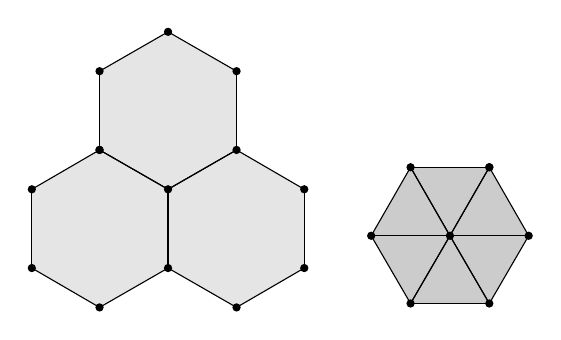
\begin{tikzpicture}[line cap=round,line join=round,>=triangle 45,x=1.0cm,y=1.0cm]
\fill[fill=black,fill opacity=0.1] (2,1) -- (2,2) -- (1.13,2.5) --
(0.27,2) -- (0.27,1) -- (1.13,0.5) -- cycle; \fill[fill=black,fill
opacity=0.1] (2,2) -- (2,1) -- (2.87,0.5) -- (3.73,1) -- (3.73,2) --
(2.87,2.5) -- cycle; \fill[fill=black,fill opacity=0.1] (2,2) --
(2.87,2.5) -- (2.87,3.5) -- (2,4) -- (1.13,3.5) -- (1.13,2.5) --
cycle; \fill[fill=black,fill opacity=0.2] (6.08,2.28) -- (5.08,2.28)
-- (5.58,1.41) -- cycle; \fill[fill=black,fill opacity=0.2]
(5.58,1.41) -- (5.08,2.28) -- (4.58,1.41) -- cycle;
\fill[fill=black,fill opacity=0.2] (5.58,1.41) -- (4.58,1.41) --
(5.08,0.55) -- cycle; \fill[fill=black,fill opacity=0.2] (5.58,1.41)
-- (5.08,0.55) -- (6.08,0.55) -- cycle; \fill[fill=black,fill
opacity=0.2] (5.58,1.41) -- (6.08,0.55) -- (6.58,1.41) -- cycle;
\fill[fill=black,fill opacity=0.2] (5.58,1.41) -- (6.58,1.41) --
(6.08,2.28) -- cycle; \draw (2,1)-- (2,2); \draw (2,2)-- (1.13,2.5);
\draw (1.13,2.5)-- (0.27,2); \draw (0.27,2)-- (0.27,1); \draw
(0.27,1)-- (1.13,0.5); \draw (1.13,0.5)-- (2,1); \draw (2,2)--
(2,1); \draw (2,1)-- (2.87,0.5); \draw (2.87,0.5)-- (3.73,1); \draw
(3.73,1)-- (3.73,2); \draw (3.73,2)-- (2.87,2.5); \draw (2.87,2.5)--
(2,2); \draw (2,2)-- (2.87,2.5); \draw (2.87,2.5)-- (2.87,3.5);
\draw (2.87,3.5)-- (2,4); \draw (2,4)-- (1.13,3.5); \draw
(1.13,3.5)-- (1.13,2.5); \draw (1.13,2.5)-- (2,2); \draw
(6.08,2.28)-- (5.08,2.28); \draw (5.08,2.28)-- (5.58,1.41); \draw
(5.58,1.41)-- (6.08,2.28); \draw (5.58,1.41)-- (5.08,2.28); \draw
(5.08,2.28)-- (4.58,1.41); \draw (4.58,1.41)-- (5.58,1.41); \draw
(5.58,1.41)-- (4.58,1.41); \draw (4.58,1.41)-- (5.08,0.55); \draw
(5.08,0.55)-- (5.58,1.41); \draw (5.58,1.41)-- (5.08,0.55); \draw
(5.08,0.55)-- (6.08,0.55); \draw (6.08,0.55)-- (5.58,1.41); \draw
(5.58,1.41)-- (6.08,0.55); \draw (6.08,0.55)-- (6.58,1.41); \draw
(6.58,1.41)-- (5.58,1.41); \draw (5.58,1.41)-- (6.58,1.41); \draw
(6.58,1.41)-- (6.08,2.28); \draw (6.08,2.28)-- (5.58,1.41);
\begin{scriptsize}
\fill [color=black] (2,1) circle (1.5pt); \fill [color=black] (2,2)
circle (1.5pt); \fill [color=black] (1.13,2.5) circle (1.5pt); \fill
[color=black] (0.27,2) circle (1.5pt); \fill [color=black] (0.27,1)
circle (1.5pt); \fill [color=black] (1.13,0.5) circle (1.5pt); \fill
[color=black] (2.87,0.5) circle (1.5pt); \fill [color=black]
(3.73,1) circle (1.5pt); \fill [color=black] (3.73,2) circle
(1.5pt); \fill [color=black] (2.87,2.5) circle (1.5pt); \fill
[color=black] (2.87,3.5) circle (1.5pt); \fill [color=black] (2,4)
circle (1.5pt); \fill [color=black] (1.13,3.5) circle (1.5pt); \fill
[color=black] (1.13,2.5) circle (1.5pt); \fill [color=black]
(5.08,2.28) circle (1.5pt); \fill [color=black] (6.08,2.28) circle
(1.5pt); \fill [color=black] (5.58,1.41) circle (1.5pt); \fill
[color=black] (4.58,1.41) circle (1.5pt); \fill [color=black]
(5.08,0.55) circle (1.5pt); \fill [color=black] (6.08,0.55) circle
(1.5pt); \fill [color=black] (6.58,1.41) circle (1.5pt); \fill
[color=black] (6.08,2.28) circle (1.5pt);
\end{scriptsize}
\end{tikzpicture}
        \end{center}

    Ha egy csúcs körül csak egy hatszög lenne, akkor négy háromszög kell melléje
    ($1\cdot 120^\circ + 4\cdot 60^\circ = 360^\circ$). Az egyszer\H
    ubb hivatkozás érdekében a lefedéshez hozzárendeljük a csúcsok körül
    megjelenő sokszögek
    oldalszámaiból képezett rendezett számhalmazt egy rögzített körüljárás szerint.
    Így az előbbi lefödéshez hozzárendelhetjük a
    $(6,3,3,3,3)$ rendezett szám ötöst. Egy ilyen csúcspont
    látható a következő ábrán:
   \begin{center}
    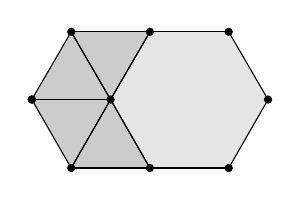
\begin{tikzpicture}[line cap=round,line join=round,>=triangle 45,x=1.0cm,y=1.0cm]
\fill[fill=black,fill opacity=0.1] (2,1) -- (3,1) -- (3.5,1.87) --
(3,2.73) -- (2,2.73) -- (1.5,1.87) -- cycle; \fill[fill=black,fill
opacity=0.2] (1.5,1.87) -- (2,2.73) -- (1,2.73) -- cycle;
\fill[fill=black,fill opacity=0.2] (2,1) -- (1.5,1.87) -- (1,1) --
cycle; \fill[fill=black,fill opacity=0.2] (1,1) -- (1.5,1.87) --
(0.5,1.87) -- cycle; \fill[fill=black,fill opacity=0.2] (1.5,1.87)
-- (1,2.73) -- (0.5,1.87) -- cycle; \draw (2,1)-- (3,1); \draw
(3,1)-- (3.5,1.87); \draw (3.5,1.87)-- (3,2.73); \draw (3,2.73)--
(2,2.73); \draw (2,2.73)-- (1.5,1.87); \draw (1.5,1.87)-- (2,1);
\draw (1.5,1.87)-- (2,2.73); \draw (2,2.73)-- (1,2.73); \draw
(1,2.73)-- (1.5,1.87); \draw (2,1)-- (1.5,1.87); \draw (1.5,1.87)--
(1,1); \draw (1,1)-- (2,1); \draw (1,1)-- (1.5,1.87); \draw
(1.5,1.87)-- (0.5,1.87); \draw (0.5,1.87)-- (1,1); \draw
(1.5,1.87)-- (1,2.73); \draw (1,2.73)-- (0.5,1.87); \draw
(0.5,1.87)-- (1.5,1.87);
\begin{scriptsize}
\fill [color=black] (2,1) circle (1.5pt); \fill [color=black] (3,1)
circle (1.5pt); \fill [color=black] (3.5,1.87) circle (1.5pt); \fill
[color=black] (3,2.73) circle (1.5pt); \fill [color=black] (2,2.73)
circle (1.5pt); \fill [color=black] (1.5,1.87) circle (1.5pt); \fill
[color=black] (1,2.73) circle (1.5pt); \fill [color=black] (1,1)
circle (1.5pt); \fill [color=black] (0.5,1.87) circle (1.5pt); \fill
[color=black] (0.5,1.87) circle (1.5pt);
\end{scriptsize}
\end{tikzpicture}
    \end{center}


Szabályos lefödés csak a következő módon
készíthető:
\begin{center}
    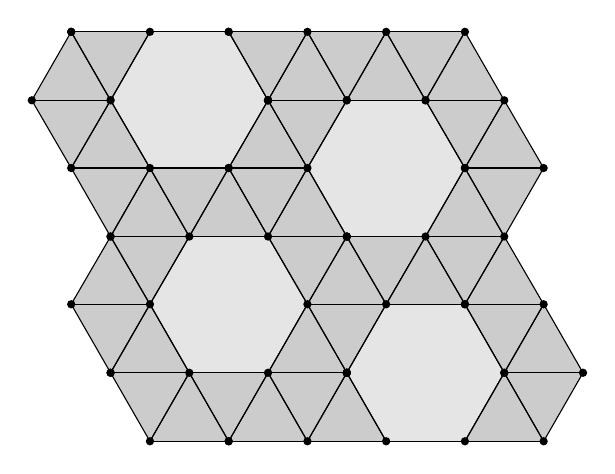
\begin{tikzpicture}[line cap=round,line join=round,>=triangle 45,x=1.0cm,y=1.0cm]
\fill[fill=black,fill opacity=0.1] (2,1) -- (3,1) -- (3.5,1.87) --
(3,2.73) -- (2,2.73) -- (1.5,1.87) -- cycle; \fill[fill=black,fill
opacity=0.2] (2,2.73) -- (3,2.73) -- (2.5,3.6) -- cycle;
\fill[fill=black,fill opacity=0.2] (1.5,1.87) -- (2,2.73) --
(1,2.73) -- cycle; \fill[fill=black,fill opacity=0.2] (2,1) --
(1.5,1.87) -- (1,1) -- cycle; \fill[fill=black,fill opacity=0.2]
(3,1) -- (2,1) -- (2.5,0.13) -- cycle; \fill[fill=black,fill
opacity=0.2] (3.5,1.87) -- (3,1) -- (4,1) -- cycle;
\fill[fill=black,fill opacity=0.2] (3,2.73) -- (3.5,1.87) --
(4,2.73) -- cycle; \fill[fill=black,fill opacity=0.2] (3,2.73) --
(4,2.73) -- (3.5,3.6) -- cycle; \fill[fill=black,fill opacity=0.2]
(3,2.73) -- (3.5,3.6) -- (2.5,3.6) -- cycle; \fill[fill=black,fill
opacity=0.2] (2,2.73) -- (2.5,3.6) -- (1.5,3.6) -- cycle;
\fill[fill=black,fill opacity=0.2] (2,2.73) -- (1.5,3.6) -- (1,2.73)
-- cycle; \fill[fill=black,fill opacity=0.2] (1.5,1.87) -- (1,2.73)
-- (0.5,1.87) -- cycle; \fill[fill=black,fill opacity=0.2]
(1.5,1.87) -- (0.5,1.87) -- (1,1) -- cycle; \fill[fill=black,fill
opacity=0.2] (2,1) -- (1,1) -- (1.5,0.13) -- cycle;
\fill[fill=black,fill opacity=0.2] (2,1) -- (1.5,0.13) -- (2.5,0.13)
-- cycle; \fill[fill=black,fill opacity=0.2] (3,1) -- (2.5,0.13) --
(3.5,0.13) -- cycle; \fill[fill=black,fill opacity=0.2] (3,1) --
(3.5,0.13) -- (4,1) -- cycle; \fill[fill=black,fill opacity=0.2]
(3.5,1.87) -- (4,1) -- (4.5,1.87) -- cycle; \fill[fill=black,fill
opacity=0.2] (3.5,1.87) -- (4.5,1.87) -- (4,2.73) -- cycle;
\fill[fill=black,fill opacity=0.1] (3.5,3.6) -- (4,2.73) -- (5,2.73)
-- (5.5,3.6) -- (5,4.46) -- (4,4.46) -- cycle; \fill[fill=black,fill
opacity=0.2] (4.5,1.87) -- (5,2.73) -- (4,2.73) -- cycle;
\fill[fill=black,fill opacity=0.2] (5,2.73) -- (4.5,1.87) --
(5.5,1.87) -- cycle; \fill[fill=black,fill opacity=0.1] (5.5,1.87)
-- (4.5,1.87) -- (4,1) -- (4.5,0.13) -- (5.5,0.13) -- (6,1) --
cycle; \fill[fill=black,fill opacity=0.2] (3.5,0.13) -- (4.5,0.13)
-- (4,1) -- cycle; \fill[fill=black,fill opacity=0.2] (5,2.73) --
(5.5,1.87) -- (6,2.73) -- cycle; \fill[fill=black,fill opacity=0.2]
(5,2.73) -- (6,2.73) -- (5.5,3.6) -- cycle; \fill[fill=black,fill
opacity=0.2] (5.5,3.6) -- (6,2.73) -- (6.5,3.6) -- cycle;
\fill[fill=black,fill opacity=0.2] (5.5,3.6) -- (6.5,3.6) --
(6,4.46) -- cycle; \fill[fill=black,fill opacity=0.2] (5.5,3.6) --
(6,4.46) -- (5,4.46) -- cycle; \fill[fill=black,fill opacity=0.2]
(5,4.46) -- (6,4.46) -- (5.5,5.33) -- cycle; \fill[fill=black,fill
opacity=0.2] (5,4.46) -- (5.5,5.33) -- (4.5,5.33) -- cycle;
\fill[fill=black,fill opacity=0.2] (5,4.46) -- (4.5,5.33) --
(4,4.46) -- cycle; \fill[fill=black,fill opacity=0.2] (4,4.46) --
(4.5,5.33) -- (3.5,5.33) -- cycle; \fill[fill=black,fill
opacity=0.2] (4,4.46) -- (3.5,5.33) -- (3,4.46) -- cycle;
\fill[fill=black,fill opacity=0.2] (3.5,3.6) -- (4,4.46) -- (3,4.46)
-- cycle; \fill[fill=black,fill opacity=0.2] (2.5,3.6) -- (3.5,3.6)
-- (3,4.46) -- cycle; \fill[fill=black,fill opacity=0.1] (1.5,3.6)
-- (2.5,3.6) -- (3,4.46) -- (2.5,5.33) -- (1.5,5.33) -- (1,4.46) --
cycle; \fill[fill=black,fill opacity=0.2] (3,4.46) -- (3.5,5.33) --
(2.5,5.33) -- cycle; \fill[fill=black,fill opacity=0.2] (6,2.73) --
(5.5,1.87) -- (6.5,1.87) -- cycle; \fill[fill=black,fill
opacity=0.2] (6,1) -- (6.5,1.87) -- (5.5,1.87) -- cycle;
\fill[fill=black,fill opacity=0.2] (6.5,1.87) -- (6,1) -- (7,1) --
cycle; \fill[fill=black,fill opacity=0.2] (7,1) -- (6,1) --
(6.5,0.13) -- cycle; \fill[fill=black,fill opacity=0.2] (5.5,0.13)
-- (6.5,0.13) -- (6,1) -- cycle; \fill[fill=black,fill opacity=0.2]
(1,2.73) -- (1.5,3.6) -- (0.5,3.6) -- cycle; \fill[fill=black,fill
opacity=0.2] (0.5,3.6) -- (1.5,3.6) -- (1,4.46) -- cycle;
\fill[fill=black,fill opacity=0.2] (0.5,3.6) -- (1,4.46) -- (0,4.46)
-- cycle; \fill[fill=black,fill opacity=0.2] (0,4.46) -- (1,4.46) --
(0.5,5.33) -- cycle; \fill[fill=black,fill opacity=0.2] (1,4.46) --
(1.5,5.33) -- (0.5,5.33) -- cycle; \draw (2,1)-- (3,1); \draw
(3,1)-- (3.5,1.87); \draw (3.5,1.87)-- (3,2.73); \draw (3,2.73)--
(2,2.73); \draw (2,2.73)-- (1.5,1.87); \draw (1.5,1.87)-- (2,1);
\draw (2,2.73)-- (3,2.73); \draw (3,2.73)-- (2.5,3.6); \draw
(2.5,3.6)-- (2,2.73); \draw (1.5,1.87)-- (2,2.73); \draw (2,2.73)--
(1,2.73); \draw (1,2.73)-- (1.5,1.87); \draw (2,1)-- (1.5,1.87);
\draw (1.5,1.87)-- (1,1); \draw (1,1)-- (2,1); \draw (3,1)-- (2,1);
\draw (2,1)-- (2.5,0.13); \draw (2.5,0.13)-- (3,1); \draw
(3.5,1.87)-- (3,1); \draw (3,1)-- (4,1); \draw (4,1)-- (3.5,1.87);
\draw (3,2.73)-- (3.5,1.87); \draw (3.5,1.87)-- (4,2.73); \draw
(4,2.73)-- (3,2.73); \draw (3,2.73)-- (4,2.73); \draw (4,2.73)--
(3.5,3.6); \draw (3.5,3.6)-- (3,2.73); \draw (3,2.73)-- (3.5,3.6);
\draw (3.5,3.6)-- (2.5,3.6); \draw (2.5,3.6)-- (3,2.73); \draw
(2,2.73)-- (2.5,3.6); \draw (2.5,3.6)-- (1.5,3.6); \draw (1.5,3.6)--
(2,2.73); \draw (2,2.73)-- (1.5,3.6); \draw (1.5,3.6)-- (1,2.73);
\draw (1,2.73)-- (2,2.73); \draw (1.5,1.87)-- (1,2.73); \draw
(1,2.73)-- (0.5,1.87); \draw (0.5,1.87)-- (1.5,1.87); \draw
(1.5,1.87)-- (0.5,1.87); \draw (0.5,1.87)-- (1,1); \draw (1,1)--
(1.5,1.87); \draw (2,1)-- (1,1); \draw (1,1)-- (1.5,0.13); \draw
(1.5,0.13)-- (2,1); \draw (2,1)-- (1.5,0.13); \draw (1.5,0.13)--
(2.5,0.13); \draw (2.5,0.13)-- (2,1); \draw (3,1)-- (2.5,0.13);
\draw (2.5,0.13)-- (3.5,0.13); \draw (3.5,0.13)-- (3,1); \draw
(3,1)-- (3.5,0.13); \draw (3.5,0.13)-- (4,1); \draw (4,1)-- (3,1);
\draw (3.5,1.87)-- (4,1); \draw (4,1)-- (4.5,1.87); \draw
(4.5,1.87)-- (3.5,1.87); \draw (3.5,1.87)-- (4.5,1.87); \draw
(4.5,1.87)-- (4,2.73); \draw (4,2.73)-- (3.5,1.87); \draw
(3.5,3.6)-- (4,2.73); \draw (4,2.73)-- (5,2.73); \draw (5,2.73)--
(5.5,3.6); \draw (5.5,3.6)-- (5,4.46); \draw (5,4.46)-- (4,4.46);
\draw (4,4.46)-- (3.5,3.6); \draw (4.5,1.87)-- (5,2.73); \draw
(5,2.73)-- (4,2.73); \draw (4,2.73)-- (4.5,1.87); \draw (5,2.73)--
(4.5,1.87); \draw (4.5,1.87)-- (5.5,1.87); \draw (5.5,1.87)--
(5,2.73); \draw (5.5,1.87)-- (4.5,1.87); \draw (4.5,1.87)-- (4,1);
\draw (4,1)-- (4.5,0.13); \draw (4.5,0.13)-- (5.5,0.13); \draw
(5.5,0.13)-- (6,1); \draw (6,1)-- (5.5,1.87); \draw (3.5,0.13)--
(4.5,0.13); \draw (4.5,0.13)-- (4,1); \draw (4,1)-- (3.5,0.13);
\draw (5,2.73)-- (5.5,1.87); \draw (5.5,1.87)-- (6,2.73); \draw
(6,2.73)-- (5,2.73); \draw (5,2.73)-- (6,2.73); \draw (6,2.73)--
(5.5,3.6); \draw (5.5,3.6)-- (5,2.73); \draw (5.5,3.6)-- (6,2.73);
\draw (6,2.73)-- (6.5,3.6); \draw (6.5,3.6)-- (5.5,3.6); \draw
(5.5,3.6)-- (6.5,3.6); \draw (6.5,3.6)-- (6,4.46); \draw (6,4.46)--
(5.5,3.6); \draw (5.5,3.6)-- (6,4.46); \draw (6,4.46)-- (5,4.46);
\draw (5,4.46)-- (5.5,3.6); \draw (5,4.46)-- (6,4.46); \draw
(6,4.46)-- (5.5,5.33); \draw (5.5,5.33)-- (5,4.46); \draw (5,4.46)--
(5.5,5.33); \draw (5.5,5.33)-- (4.5,5.33); \draw (4.5,5.33)--
(5,4.46); \draw (5,4.46)-- (4.5,5.33); \draw (4.5,5.33)-- (4,4.46);
\draw (4,4.46)-- (5,4.46); \draw (4,4.46)-- (4.5,5.33); \draw
(4.5,5.33)-- (3.5,5.33); \draw (3.5,5.33)-- (4,4.46); \draw
(4,4.46)-- (3.5,5.33); \draw (3.5,5.33)-- (3,4.46); \draw (3,4.46)--
(4,4.46); \draw (3.5,3.6)-- (4,4.46); \draw (4,4.46)-- (3,4.46);
\draw (3,4.46)-- (3.5,3.6); \draw (2.5,3.6)-- (3.5,3.6); \draw
(3.5,3.6)-- (3,4.46); \draw (3,4.46)-- (2.5,3.6); \draw (1.5,3.6)--
(2.5,3.6); \draw (2.5,3.6)-- (3,4.46); \draw (3,4.46)-- (2.5,5.33);
\draw (2.5,5.33)-- (1.5,5.33); \draw (1.5,5.33)-- (1,4.46); \draw
(1,4.46)-- (1.5,3.6); \draw (3,4.46)-- (3.5,5.33); \draw
(3.5,5.33)-- (2.5,5.33); \draw (2.5,5.33)-- (3,4.46); \draw
(6,2.73)-- (5.5,1.87); \draw (5.5,1.87)-- (6.5,1.87); \draw
(6.5,1.87)-- (6,2.73); \draw (6,1)-- (6.5,1.87); \draw (6.5,1.87)--
(5.5,1.87); \draw (5.5,1.87)-- (6,1); \draw (6.5,1.87)-- (6,1);
\draw (6,1)-- (7,1); \draw (7,1)-- (6.5,1.87); \draw (7,1)-- (6,1);
\draw (6,1)-- (6.5,0.13); \draw (6.5,0.13)-- (7,1); \draw
(5.5,0.13)-- (6.5,0.13); \draw (6.5,0.13)-- (6,1); \draw (6,1)--
(5.5,0.13); \draw (1,2.73)-- (1.5,3.6); \draw (1.5,3.6)-- (0.5,3.6);
\draw (0.5,3.6)-- (1,2.73); \draw (0.5,3.6)-- (1.5,3.6); \draw
(1.5,3.6)-- (1,4.46); \draw (1,4.46)-- (0.5,3.6); \draw (0.5,3.6)--
(1,4.46); \draw (1,4.46)-- (0,4.46); \draw (0,4.46)-- (0.5,3.6);
\draw (0,4.46)-- (1,4.46); \draw (1,4.46)-- (0.5,5.33); \draw
(0.5,5.33)-- (0,4.46); \draw (1,4.46)-- (1.5,5.33); \draw
(1.5,5.33)-- (0.5,5.33); \draw (0.5,5.33)-- (1,4.46);
\begin{scriptsize}
\fill [color=black] (2,1) circle (1.5pt); \fill [color=black] (3,1)
circle (1.5pt); \fill [color=black] (3.5,1.87) circle (1.5pt); \fill
[color=black] (3,2.73) circle (1.5pt); \fill [color=black] (2,2.73)
circle (1.5pt); \fill [color=black] (1.5,1.87) circle (1.5pt); \fill
[color=black] (2.5,3.6) circle (1.5pt); \fill [color=black] (1,2.73)
circle (1.5pt); \fill [color=black] (1,1) circle (1.5pt); \fill
[color=black] (2.5,0.13) circle (1.5pt); \fill [color=black] (4,1)
circle (1.5pt); \fill [color=black] (4,2.73) circle (1.5pt); \fill
[color=black] (3.5,3.6) circle (1.5pt); \fill [color=black]
(2.5,3.6) circle (1.5pt); \fill [color=black] (1.5,3.6) circle
(1.5pt); \fill [color=black] (1,2.73) circle (1.5pt); \fill
[color=black] (0.5,1.87) circle (1.5pt); \fill [color=black] (1,1)
circle (1.5pt); \fill [color=black] (1.5,0.13) circle (1.5pt); \fill
[color=black] (2.5,0.13) circle (1.5pt); \fill [color=black]
(3.5,0.13) circle (1.5pt); \fill [color=black] (4,1) circle (1.5pt);
\fill [color=black] (4.5,1.87) circle (1.5pt); \fill [color=black]
(4,2.73) circle (1.5pt); \fill [color=black] (5,2.73) circle
(1.5pt); \fill [color=black] (5.5,3.6) circle (1.5pt); \fill
[color=black] (5,4.46) circle (1.5pt); \fill [color=black] (4,4.46)
circle (1.5pt); \fill [color=black] (4,2.73) circle (1.5pt); \fill
[color=black] (5.5,1.87) circle (1.5pt); \fill [color=black] (4,1)
circle (1.5pt); \fill [color=black] (4.5,0.13) circle (1.5pt); \fill
[color=black] (5.5,0.13) circle (1.5pt); \fill [color=black] (6,1)
circle (1.5pt); \fill [color=black] (4,1) circle (1.5pt); \fill
[color=black] (6,2.73) circle (1.5pt); \fill [color=black] (5.5,3.6)
circle (1.5pt); \fill [color=black] (6.5,3.6) circle (1.5pt); \fill
[color=black] (6,4.46) circle (1.5pt); \fill [color=black] (5,4.46)
circle (1.5pt); \fill [color=black] (5.5,5.33) circle (1.5pt); \fill
[color=black] (4.5,5.33) circle (1.5pt); \fill [color=black]
(4,4.46) circle (1.5pt); \fill [color=black] (3.5,5.33) circle
(1.5pt); \fill [color=black] (3,4.46) circle (1.5pt); \fill
[color=black] (3,4.46) circle (1.5pt); \fill [color=black] (3,4.46)
circle (1.5pt); \fill [color=black] (3,4.46) circle (1.5pt); \fill
[color=black] (2.5,5.33) circle (1.5pt); \fill [color=black]
(1.5,5.33) circle (1.5pt); \fill [color=black] (1,4.46) circle
(1.5pt); \fill [color=black] (2.5,5.33) circle (1.5pt); \fill
[color=black] (6.5,1.87) circle (1.5pt); \fill [color=black]
(5.5,1.87) circle (1.5pt); \fill [color=black] (7,1) circle (1.5pt);
\fill [color=black] (6.5,0.13) circle (1.5pt); \fill [color=black]
(6,1) circle (1.5pt); \fill [color=black] (0.5,3.6) circle (1.5pt);
\fill [color=black] (1,4.46) circle (1.5pt); \fill [color=black]
(0,4.46) circle (1.5pt); \fill [color=black] (0.5,5.33) circle
(1.5pt); \fill [color=black] (0.5,5.33) circle (1.5pt);
\end{scriptsize}
\end{tikzpicture}
\end{center}
Ha egy csúcs körül két hatszög lenne, akkor két
háromszög kell hozzá ($2\cdot 120^\circ + 2\cdot 60^\circ =
360^\circ$). Ez esetben kétféle csúcs lehetséges:
$(6,3,6,3)$, illetve $(6,6,3,3)$.
\begin{itemize}
    \item A $(6,3,6,3)$ esetben egy csúcs körüli elhelyezés látható a bal oldalon,
    míg a szabályos lefödés a egy része jobb oldalon:

    \begin{center}
    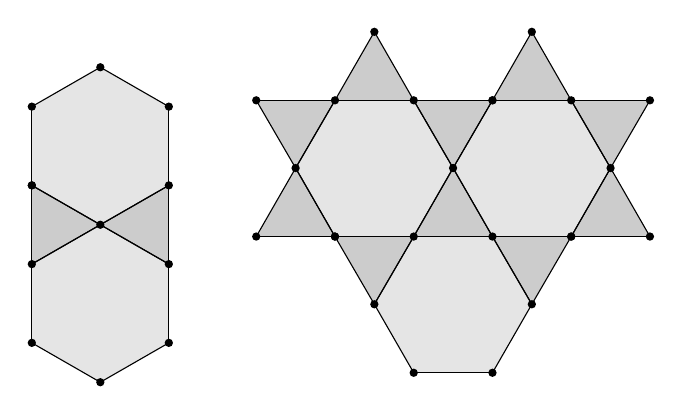
\begin{tikzpicture}[line cap=round,line join=round,>=triangle 45,x=1.0cm,y=1.0cm]
\fill[fill=black,fill opacity=0.1] (7.51,-0.85) -- (8.51,-0.85) --
(9.01,0.02) -- (8.51,0.88) -- (7.51,0.88) -- (7.01,0.02) -- cycle;
\fill[fill=black,fill opacity=0.2] (7.51,0.88) -- (8.51,0.88) --
(8.01,1.75) -- cycle; \fill[fill=black,fill opacity=0.2] (7.01,0.02)
-- (7.51,0.88) -- (6.51,0.88) -- cycle; \fill[fill=black,fill
opacity=0.2] (8.51,0.88) -- (9.01,0.02) -- (9.51,0.88) -- cycle;
\fill[fill=black,fill opacity=0.1] (8.01,1.75) -- (8.51,0.88) --
(9.51,0.88) -- (10.01,1.75) -- (9.51,2.61) -- (8.51,2.61) -- cycle;
\fill[fill=black,fill opacity=0.1] (7.51,0.88) -- (8.01,1.75) --
(7.51,2.61) -- (6.51,2.61) -- (6.01,1.75) -- (6.51,0.88) -- cycle;
\fill[fill=black,fill opacity=0.2] (6.51,0.88) -- (6.01,1.75) --
(5.51,0.88) -- cycle; \fill[fill=black,fill opacity=0.2] (6.01,1.75)
-- (6.51,2.61) -- (5.51,2.61) -- cycle; \fill[fill=black,fill
opacity=0.2] (6.51,2.61) -- (7.51,2.61) -- (7.01,3.48) -- cycle;
\fill[fill=black,fill opacity=0.2] (7.51,2.61) -- (8.01,1.75) --
(8.51,2.61) -- cycle; \fill[fill=black,fill opacity=0.2] (8.51,2.61)
-- (9.51,2.61) -- (9.01,3.48) -- cycle; \fill[fill=black,fill
opacity=0.2] (9.51,2.61) -- (10.01,1.75) -- (10.51,2.61) -- cycle;
\fill[fill=black,fill opacity=0.2] (10.01,1.75) -- (9.51,0.88) --
(10.51,0.88) -- cycle; \fill[fill=black,fill opacity=0.1]
(4.4,-0.47) -- (4.4,0.53) -- (3.53,1.03) -- (2.66,0.53) --
(2.66,-0.47) -- (3.53,-0.97) -- cycle; \fill[fill=black,fill
opacity=0.2] (3.53,1.03) -- (4.4,0.53) -- (4.4,1.53) -- cycle;
\fill[fill=black,fill opacity=0.2] (2.66,0.53) -- (3.53,1.03) --
(2.66,1.53) -- cycle; \fill[fill=black,fill opacity=0.1] (3.53,1.03)
-- (4.4,1.53) -- (4.4,2.53) -- (3.53,3.03) -- (2.66,2.53) --
(2.66,1.53) -- cycle; \draw (7.51,-0.85)-- (8.51,-0.85); \draw
(8.51,-0.85)-- (9.01,0.02); \draw (9.01,0.02)-- (8.51,0.88); \draw
(8.51,0.88)-- (7.51,0.88); \draw (7.51,0.88)-- (7.01,0.02); \draw
(7.01,0.02)-- (7.51,-0.85); \draw (7.51,0.88)-- (8.51,0.88); \draw
(8.51,0.88)-- (8.01,1.75); \draw (8.01,1.75)-- (7.51,0.88); \draw
(7.01,0.02)-- (7.51,0.88); \draw (7.51,0.88)-- (6.51,0.88); \draw
(6.51,0.88)-- (7.01,0.02); \draw (8.51,0.88)-- (9.01,0.02); \draw
(9.01,0.02)-- (9.51,0.88); \draw (9.51,0.88)-- (8.51,0.88); \draw
(8.01,1.75)-- (8.51,0.88); \draw (8.51,0.88)-- (9.51,0.88); \draw
(9.51,0.88)-- (10.01,1.75); \draw (10.01,1.75)-- (9.51,2.61); \draw
(9.51,2.61)-- (8.51,2.61); \draw (8.51,2.61)-- (8.01,1.75); \draw
(7.51,0.88)-- (8.01,1.75); \draw (8.01,1.75)-- (7.51,2.61); \draw
(7.51,2.61)-- (6.51,2.61); \draw (6.51,2.61)-- (6.01,1.75); \draw
(6.01,1.75)-- (6.51,0.88); \draw (6.51,0.88)-- (7.51,0.88); \draw
(6.51,0.88)-- (6.01,1.75); \draw (6.01,1.75)-- (5.51,0.88); \draw
(5.51,0.88)-- (6.51,0.88); \draw (6.01,1.75)-- (6.51,2.61); \draw
(6.51,2.61)-- (5.51,2.61); \draw (5.51,2.61)-- (6.01,1.75); \draw
(6.51,2.61)-- (7.51,2.61); \draw (7.51,2.61)-- (7.01,3.48); \draw
(7.01,3.48)-- (6.51,2.61); \draw (7.51,2.61)-- (8.01,1.75); \draw
(8.01,1.75)-- (8.51,2.61); \draw (8.51,2.61)-- (7.51,2.61); \draw
(8.51,2.61)-- (9.51,2.61); \draw (9.51,2.61)-- (9.01,3.48); \draw
(9.01,3.48)-- (8.51,2.61); \draw (9.51,2.61)-- (10.01,1.75); \draw
(10.01,1.75)-- (10.51,2.61); \draw (10.51,2.61)-- (9.51,2.61); \draw
(10.01,1.75)-- (9.51,0.88); \draw (9.51,0.88)-- (10.51,0.88); \draw
(10.51,0.88)-- (10.01,1.75); \draw (4.4,-0.47)-- (4.4,0.53); \draw
(4.4,0.53)-- (3.53,1.03); \draw (3.53,1.03)-- (2.66,0.53); \draw
(2.66,0.53)-- (2.66,-0.47); \draw (2.66,-0.47)-- (3.53,-0.97); \draw
(3.53,-0.97)-- (4.4,-0.47); \draw (3.53,1.03)-- (4.4,0.53); \draw
(4.4,0.53)-- (4.4,1.53); \draw (4.4,1.53)-- (3.53,1.03); \draw
(2.66,0.53)-- (3.53,1.03); \draw (3.53,1.03)-- (2.66,1.53); \draw
(2.66,1.53)-- (2.66,0.53); \draw (3.53,1.03)-- (4.4,1.53); \draw
(4.4,1.53)-- (4.4,2.53); \draw (4.4,2.53)-- (3.53,3.03); \draw
(3.53,3.03)-- (2.66,2.53); \draw (2.66,2.53)-- (2.66,1.53); \draw
(2.66,1.53)-- (3.53,1.03);
\begin{scriptsize}
\fill [color=black] (7.51,-0.85) circle (1.5pt); \fill [color=black]
(8.51,-0.85) circle (1.5pt); \fill [color=black] (9.01,0.02) circle
(1.5pt); \fill [color=black] (8.51,0.88) circle (1.5pt); \fill
[color=black] (7.51,0.88) circle (1.5pt); \fill [color=black]
(7.01,0.02) circle (1.5pt); \fill [color=black] (8.01,1.75) circle
(1.5pt); \fill [color=black] (6.51,0.88) circle (1.5pt); \fill
[color=black] (9.51,0.88) circle (1.5pt); \fill [color=black]
(9.51,0.88) circle (1.5pt); \fill [color=black] (10.01,1.75) circle
(1.5pt); \fill [color=black] (9.51,2.61) circle (1.5pt); \fill
[color=black] (8.51,2.61) circle (1.5pt); \fill [color=black]
(7.51,2.61) circle (1.5pt); \fill [color=black] (6.51,2.61) circle
(1.5pt); \fill [color=black] (6.01,1.75) circle (1.5pt); \fill
[color=black] (6.51,0.88) circle (1.5pt); \fill [color=black]
(5.51,0.88) circle (1.5pt); \fill [color=black] (5.51,2.61) circle
(1.5pt); \fill [color=black] (7.01,3.48) circle (1.5pt); \fill
[color=black] (8.51,2.61) circle (1.5pt); \fill [color=black]
(9.01,3.48) circle (1.5pt); \fill [color=black] (10.51,2.61) circle
(1.5pt); \fill [color=black] (10.51,0.88) circle (1.5pt); \fill
[color=black] (4.4,-0.47) circle (1.5pt); \fill [color=black]
(4.4,0.53) circle (1.5pt); \fill [color=black] (3.53,1.03) circle
(1.5pt); \fill [color=black] (2.66,0.53) circle (1.5pt); \fill
[color=black] (2.66,-0.47) circle (1.5pt); \fill [color=black]
(3.53,-0.97) circle (1.5pt); \fill [color=black] (4.4,1.53) circle
(1.5pt); \fill [color=black] (2.66,1.53) circle (1.5pt); \fill
[color=black] (4.4,2.53) circle (1.5pt); \fill [color=black]
(3.53,3.03) circle (1.5pt); \fill [color=black] (2.66,2.53) circle
(1.5pt); \fill [color=black] (2.66,1.53) circle (1.5pt);
\end{scriptsize}
\end{tikzpicture}   \end{center}

    \item A $(6,6,3,3)$ esetben egy csúcs körüli elhelyezést tüntettünk fel a következő bal oldali ábrán.
    \begin{center}
    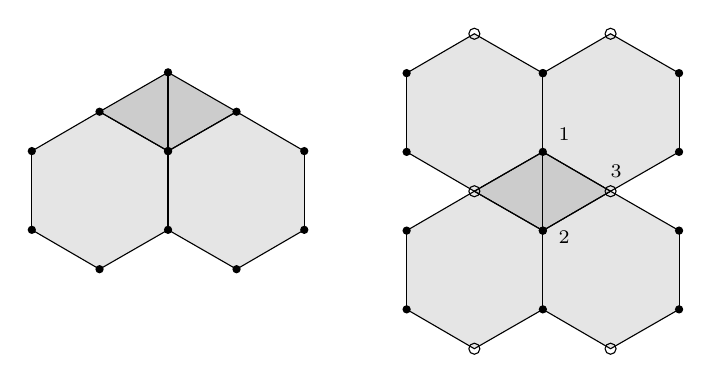
\begin{tikzpicture}[line cap=round,line join=round,>=triangle 45,x=1.0cm,y=1.0cm]
\fill[fill=black,fill opacity=0.1] (2,0) -- (2,1) -- (1.13,1.5) --
(0.27,1) -- (0.27,0) -- (1.13,-0.5) -- cycle; \fill[fill=black,fill
opacity=0.1] (2,1) -- (2,0) -- (2.87,-0.5) -- (3.73,0) -- (3.73,1)
-- (2.87,1.5) -- cycle; \fill[fill=black,fill opacity=0.2]
(1.13,1.5) -- (2,1) -- (2,2) -- cycle; \fill[fill=black,fill
opacity=0.2] (2.87,1.5) -- (2,2) -- (2,1) -- cycle;
\fill[fill=black,fill opacity=0.1] (6.76,-1.01) -- (6.76,-0.01) --
(5.89,0.49) -- (5.03,-0.01) -- (5.03,-1.01) -- (5.89,-1.51) --
cycle; \fill[fill=black,fill opacity=0.1] (6.76,-0.01) --
(6.76,-1.01) -- (7.62,-1.51) -- (8.49,-1.01) -- (8.49,-0.01) --
(7.62,0.49) -- cycle; \fill[fill=black,fill opacity=0.2] (5.89,0.49)
-- (6.76,-0.01) -- (6.76,0.99) -- cycle; \fill[fill=black,fill
opacity=0.2] (7.62,0.49) -- (6.76,0.99) -- (6.76,-0.01) -- cycle;
\fill[fill=black,fill opacity=0.1] (6.76,0.99) -- (7.62,0.49) --
(8.49,0.99) -- (8.49,1.99) -- (7.62,2.49) -- (6.76,1.99) -- cycle;
\fill[fill=black,fill opacity=0.1] (5.89,0.49) -- (6.76,0.99) --
(6.76,1.99) -- (5.89,2.49) -- (5.03,1.99) -- (5.03,0.99) -- cycle;
\draw (2,0)-- (2,1); \draw (2,1)-- (1.13,1.5); \draw (1.13,1.5)--
(0.27,1); \draw (0.27,1)-- (0.27,0); \draw (0.27,0)-- (1.13,-0.5);
\draw (1.13,-0.5)-- (2,0); \draw (2,1)-- (2,0); \draw (2,0)--
(2.87,-0.5); \draw (2.87,-0.5)-- (3.73,0); \draw (3.73,0)--
(3.73,1); \draw (3.73,1)-- (2.87,1.5); \draw (2.87,1.5)-- (2,1);
\draw (1.13,1.5)-- (2,1); \draw (2,1)-- (2,2); \draw (2,2)--
(1.13,1.5); \draw (2.87,1.5)-- (2,2); \draw (2,2)-- (2,1); \draw
(2,1)-- (2.87,1.5); \draw (6.76,-1.01)-- (6.76,-0.01); \draw
(6.76,-0.01)-- (5.89,0.49); \draw (5.89,0.49)-- (5.03,-0.01); \draw
(5.03,-0.01)-- (5.03,-1.01); \draw (5.03,-1.01)-- (5.89,-1.51);
\draw (5.89,-1.51)-- (6.76,-1.01); \draw (6.76,-0.01)--
(6.76,-1.01); \draw (6.76,-1.01)-- (7.62,-1.51); \draw
(7.62,-1.51)-- (8.49,-1.01); \draw (8.49,-1.01)-- (8.49,-0.01);
\draw (8.49,-0.01)-- (7.62,0.49); \draw (7.62,0.49)-- (6.76,-0.01);
\draw (5.89,0.49)-- (6.76,-0.01); \draw (6.76,-0.01)-- (6.76,0.99);
\draw (6.76,0.99)-- (5.89,0.49); \draw (7.62,0.49)-- (6.76,0.99);
\draw (6.76,0.99)-- (6.76,-0.01); \draw (6.76,-0.01)-- (7.62,0.49);
\draw (6.76,0.99)-- (7.62,0.49); \draw (7.62,0.49)-- (8.49,0.99);
\draw (8.49,0.99)-- (8.49,1.99); \draw (8.49,1.99)-- (7.62,2.49);
\draw (7.62,2.49)-- (6.76,1.99); \draw (6.76,1.99)-- (6.76,0.99);
\draw (5.89,0.49)-- (6.76,0.99); \draw (6.76,0.99)-- (6.76,1.99);
\draw (6.76,1.99)-- (5.89,2.49); \draw (5.89,2.49)-- (5.03,1.99);
\draw (5.03,1.99)-- (5.03,0.99); \draw (5.03,0.99)-- (5.89,0.49);
\begin{scriptsize}
\fill [color=black] (2,0) circle (1.5pt); \fill [color=black] (2,1)
circle (1.5pt); \fill [color=black] (1.13,1.5) circle (1.5pt); \fill
[color=black] (0.27,1) circle (1.5pt); \fill [color=black] (0.27,0)
circle (1.5pt); \fill [color=black] (1.13,-0.5) circle (1.5pt);
\fill [color=black] (2.87,-0.5) circle (1.5pt); \fill [color=black]
(3.73,0) circle (1.5pt); \fill [color=black] (3.73,1) circle
(1.5pt); \fill [color=black] (2.87,1.5) circle (1.5pt); \fill
[color=black] (2,2) circle (1.5pt); \fill [color=black] (2,1) circle
(1.5pt); \fill [color=black] (6.76,-1.01) circle (1.5pt); \fill
[color=black] (6.76,-0.01) circle (1.5pt); \draw[color=black]
(7.03,-0.1) node {$2$}; \draw [color=black] (5.89,0.49) circle
(2.0pt); \fill [color=black] (5.03,-0.01) circle (1.5pt); \fill
[color=black] (5.03,-1.01) circle (1.5pt); \draw [color=black]
(5.89,-1.51) circle (2.0pt); \draw [color=black] (7.62,-1.51) circle
(2.0pt); \fill [color=black] (8.49,-1.01) circle (1.5pt); \fill
[color=black] (8.49,-0.01) circle (1.5pt); \draw [color=black]
(7.62,0.49) circle (2.0pt); \draw[color=black] (7.69,0.74) node
{$3$}; \fill [color=black] (6.76,0.99) circle (1.5pt);
\draw[color=black] (7.03,1.21) node {$1$}; \fill [color=black]
(6.76,-0.01) circle (1.5pt); \fill [color=black] (8.49,0.99) circle
(1.5pt); \fill [color=black] (8.49,1.99) circle (1.5pt); \draw
[color=black] (7.62,2.49) circle (2.0pt); \fill [color=black]
(6.76,1.99) circle (1.5pt); \fill [color=black] (6.76,1.99) circle
(1.5pt); \draw [color=black] (5.89,2.49) circle (2.0pt); \fill
[color=black] (5.03,1.99) circle (1.5pt); \fill [color=black]
(5.03,0.99) circle (1.5pt);
\end{scriptsize}
\end{tikzpicture}
    \end{center}
    Ebben az esetben szabályos lefödés nem létezik,
    amit az előbbi ábra jobb oldala is bizonyít. Valóban, ha kiindulunk az $1$-el jelölt $(6,6,3,3)$ típusú csúcsból, akkor a $2$-es csúcs is szükségszerűen $(6,6,3,3)$  típusú lesz. Viszont ez azt jelenti, hogy a $3$-as csúcs már csak $(6,3,6,3)$ típusú lehet. Ez a folyamat folytatódik, két fajta csúcsunk lesz: a teli csúcsok típusa az ábrán $(6,6,3,3),$
    míg az üres csúcsok $(6,3,6,3)$ típusúak.
\end{itemize}
Áttérünk a  b) alpont megoldására. Vegyük fel a
következő ábrán látható szabályos lefödést és a
hozzá tartozó, nem derékszögű koordináta-rendszert.

A lefödésben szereplő hatszögek középpontjainak a
koordinátái $(2k, 2l)$ alakúak, ahol $k,l\in\mathbb{Z}$.

Az összes olyan hatszöget, amely középpontjának a
koordinátái nem $(2^k, 2^k),$ $k\in \mathbb{N}, k\geq 1$
alakúak, cseréljük ki a hatszög egyértel\-mű
háromszög-lefödésére.

\begin{center}
    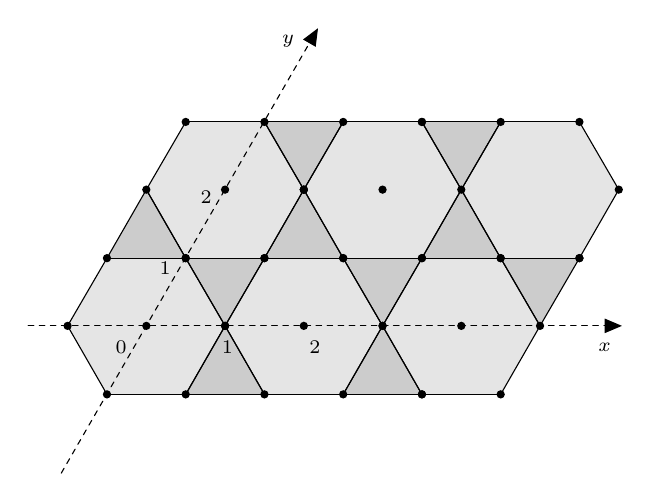
\begin{tikzpicture}[line cap=round,line join=round,>=triangle 45,x=1.0cm,y=1.0cm]
\fill[fill=black,fill opacity=0.1] (2,0) -- (3,0) -- (3.5,0.87) --
(3,1.73) -- (2,1.73) -- (1.5,0.87) -- cycle; \fill[fill=black,fill
opacity=0.2] (3,1.73) -- (3.5,0.87) -- (4,1.73) -- cycle;
\fill[fill=black,fill opacity=0.2] (3.5,0.87) -- (3,0) -- (4,0) --
cycle; \fill[fill=black,fill opacity=0.1] (4,0) -- (5,0) --
(5.5,0.87) -- (5,1.73) -- (4,1.73) -- (3.5,0.87) -- cycle;
\fill[fill=black,fill opacity=0.1] (6,0) -- (7,0) -- (7.5,0.87) --
(7,1.73) -- (6,1.73) -- (5.5,0.87) -- cycle; \fill[fill=black,fill
opacity=0.2] (5,1.73) -- (5.5,0.87) -- (6,1.73) -- cycle;
\fill[fill=black,fill opacity=0.2] (7,1.73) -- (7.5,0.87) --
(8,1.73) -- cycle; \fill[fill=black,fill opacity=0.2] (5.5,0.87) --
(5,0) -- (6,0) -- cycle; \fill[fill=black,fill opacity=0.1] (3,1.73)
-- (4,1.73) -- (4.5,2.6) -- (4,3.46) -- (3,3.46) -- (2.5,2.6) --
cycle; \fill[fill=black,fill opacity=0.1] (5,1.73) -- (6,1.73) --
(6.5,2.6) -- (6,3.46) -- (5,3.46) -- (4.5,2.6) -- cycle;
\fill[fill=black,fill opacity=0.2] (4.5,2.6) -- (4,1.73) -- (5,1.73)
-- cycle; \fill[fill=black,fill opacity=0.2] (6.5,2.6) -- (6,1.73)
-- (7,1.73) -- cycle; \fill[fill=black,fill opacity=0.2] (5,3.46) --
(4,3.46) -- (4.5,2.6) -- cycle; \fill[fill=black,fill opacity=0.2]
(2.5,2.6) -- (2,1.73) -- (3,1.73) -- cycle; \fill[fill=black,fill
opacity=0.1] (6.5,2.6) -- (7,1.73) -- (8,1.73) -- (8.5,2.6) --
(8,3.46) -- (7,3.46) -- cycle; \fill[fill=black,fill opacity=0.2]
(6.5,2.6) -- (7,3.46) -- (6,3.46) -- cycle; \draw (2,0)-- (3,0);
\draw (3,0)-- (3.5,0.87); \draw (3.5,0.87)-- (3,1.73); \draw
(3,1.73)-- (2,1.73); \draw (2,1.73)-- (1.5,0.87); \draw (1.5,0.87)--
(2,0); \draw (3,1.73)-- (3.5,0.87); \draw (3.5,0.87)-- (4,1.73);
\draw (4,1.73)-- (3,1.73); \draw (3.5,0.87)-- (3,0); \draw (3,0)--
(4,0); \draw (4,0)-- (3.5,0.87); \draw (4,0)-- (5,0); \draw (5,0)--
(5.5,0.87); \draw (5.5,0.87)-- (5,1.73); \draw (5,1.73)-- (4,1.73);
\draw (4,1.73)-- (3.5,0.87); \draw (3.5,0.87)-- (4,0); \draw (6,0)--
(7,0); \draw (7,0)-- (7.5,0.87); \draw (7.5,0.87)-- (7,1.73); \draw
(7,1.73)-- (6,1.73); \draw (6,1.73)-- (5.5,0.87); \draw (5.5,0.87)--
(6,0); \draw (5,1.73)-- (5.5,0.87); \draw (5.5,0.87)-- (6,1.73);
\draw (6,1.73)-- (5,1.73); \draw (7,1.73)-- (7.5,0.87); \draw
(7.5,0.87)-- (8,1.73); \draw (8,1.73)-- (7,1.73); \draw (5.5,0.87)--
(5,0); \draw (5,0)-- (6,0); \draw (6,0)-- (5.5,0.87); \draw
(3,1.73)-- (4,1.73); \draw (4,1.73)-- (4.5,2.6); \draw (4.5,2.6)--
(4,3.46); \draw (4,3.46)-- (3,3.46); \draw (3,3.46)-- (2.5,2.6);
\draw (2.5,2.6)-- (3,1.73); \draw (5,1.73)-- (6,1.73); \draw
(6,1.73)-- (6.5,2.6); \draw (6.5,2.6)-- (6,3.46); \draw (6,3.46)--
(5,3.46); \draw (5,3.46)-- (4.5,2.6); \draw (4.5,2.6)-- (5,1.73);
\draw (4.5,2.6)-- (4,1.73); \draw (4,1.73)-- (5,1.73); \draw
(5,1.73)-- (4.5,2.6); \draw (6.5,2.6)-- (6,1.73); \draw (6,1.73)--
(7,1.73); \draw (7,1.73)-- (6.5,2.6); \draw (5,3.46)-- (4,3.46);
\draw (4,3.46)-- (4.5,2.6); \draw (4.5,2.6)-- (5,3.46); \draw
(2.5,2.6)-- (2,1.73); \draw (2,1.73)-- (3,1.73); \draw (3,1.73)--
(2.5,2.6); \draw [->,dash pattern=on 2pt off 2pt] (1.42,-1) --
(4.68,4.65); \draw [->,dash pattern=on 2pt off 2pt] (1,0.87) --
(8.54,0.87); \draw (6.5,2.6)-- (7,1.73); \draw (7,1.73)-- (8,1.73);
\draw (8,1.73)-- (8.5,2.6); \draw (8.5,2.6)-- (8,3.46); \draw
(8,3.46)-- (7,3.46); \draw (7,3.46)-- (6.5,2.6); \draw (6.5,2.6)--
(7,3.46); \draw (7,3.46)-- (6,3.46); \draw (6,3.46)-- (6.5,2.6);
\begin{scriptsize}
\fill [color=black] (2,0) circle (1.5pt); \fill [color=black] (3,0)
circle (1.5pt); \fill [color=black] (3.5,0.87) circle (1.5pt);
\draw[color=black] (3.53,0.6) node {$1$}; \fill [color=black]
(3,1.73) circle (1.5pt); \draw[color=black] (2.74,1.6) node {$1$};
\fill [color=black] (2,1.73) circle (1.5pt); \fill [color=black]
(1.5,0.87) circle (1.5pt); \fill [color=black] (4,1.73) circle
(1.5pt); \fill [color=black] (4,0) circle (1.5pt); \fill
[color=black] (5,0) circle (1.5pt); \fill [color=black] (5.5,0.87)
circle (1.5pt); \fill [color=black] (5,1.73) circle (1.5pt); \fill
[color=black] (4,1.73) circle (1.5pt); \fill [color=black]
(3.5,0.87) circle (1.5pt); \fill [color=black] (6,0) circle (1.5pt);
\fill [color=black] (7,0) circle (1.5pt); \fill [color=black]
(7.5,0.87) circle (1.5pt); \fill [color=black] (7,1.73) circle
(1.5pt); \fill [color=black] (6,1.73) circle (1.5pt); \fill
[color=black] (5.5,0.87) circle (1.5pt); \fill [color=black]
(6,1.73) circle (1.5pt); \fill [color=black] (8,1.73) circle
(1.5pt); \fill [color=black] (6,0) circle (1.5pt); \fill
[color=black] (4.5,2.6) circle (1.5pt); \fill [color=black] (4,3.46)
circle (1.5pt); \fill [color=black] (3,3.46) circle (1.5pt); \fill
[color=black] (2.5,2.6) circle (1.5pt); \fill [color=black]
(6.5,2.6) circle (1.5pt); \fill [color=black] (6,3.46) circle
(1.5pt); \fill [color=black] (5,3.46) circle (1.5pt); \fill
[color=black] (4.5,2.6) circle (1.5pt); \fill [color=black] (5,1.73)
circle (1.5pt); \fill [color=black] (7,1.73) circle (1.5pt); \fill
[color=black] (4.5,2.6) circle (1.5pt); \fill [color=black] (3,1.73)
circle (1.5pt); \fill [color=black] (2.5,0.87) circle (1.5pt);
\draw[color=black] (2.18,0.6) node {$0$}; \fill [color=black]
(4.5,0.87) circle (1.5pt); \draw[color=black] (4.64,0.6) node {$2$};
\fill [color=black] (6.5,0.87) circle (1.5pt); \fill [color=black]
(3.5,2.6) circle (1.5pt); \draw[color=black] (3.26,2.5) node {$2$};
\fill [color=black] (5.5,2.6) circle (1.5pt); \draw[color=black]
(4.3,4.48) node {$y$}; \draw[color=black] (8.32,0.6) node {$x$};
\fill [color=black] (8,1.73) circle (1.5pt); \fill [color=black]
(8.5,2.6) circle (1.5pt); \fill [color=black] (8,3.46) circle
(1.5pt); \fill [color=black] (7,3.46) circle (1.5pt); \fill
[color=black] (6,3.46) circle (1.5pt);
\end{scriptsize}
\end{tikzpicture}
\end{center}

 Az így keletkezett
síklefödés e\-se\-tén végtelen sok olyan mintázat
létezik, amelyik véges sokszor fordul csak elő: az összes
olyan mintázat, amelyik tartalmaz két egymást követő
megmaradt hatszöget és a köztük levő szabályos
sokszögek által kitöltött alakzatot tartalmazza, csak
egyszer fordul elő mert a két hatszög középpontja közti
távolság csak egyszer fordul elő.

\textit{Megjegyzés}: Javasoljuk elolvasni mind a négy évfolyam utolsó
feladatának a meg\-ol\-dá\-sát az évfolyamok sorszámának
nö\-vek\-vő sorrendjében.




\end{document}